%%%%%%%%%%%%%%%%%%%% author.tex %%%%%%%%%%%%%%%%%%%%%%%%%%%%%%%%%%%
%
% sample root file for your "contribution" to a contributed volume
%
% Use this file as a template for your own input.
%
%%%%%%%%%%%%%%%% Springer %%%%%%%%%%%%%%%%%%%%%%%%%%%%%%%%%%


% RECOMMENDED %%%%%%%%%%%%%%%%%%%%%%%%%%%%%%%%%%%%%%%%%%%%%%%%%%%
\documentclass[graybox]{svmult}

% choose options for [] as required from the list
% in the Reference Guide

\usepackage{type1cm}        % activate if the above 3 fonts are
                            % not available on your system
%
\usepackage{makeidx}         % allows index generation
\usepackage{graphicx}        % standard LaTeX graphics tool
                             % when including figure files
\usepackage{multicol}        % used for the two-column index
\usepackage[bottom]{footmisc}% places footnotes at page bottom


\usepackage{newtxtext}       % 
\usepackage{newtxmath}       % selects Times Roman as basic font

% see the list of further useful packages
% in the Reference Guide

\makeindex             % used for the subject index
                       % please use the style svind.ist with
                       % your makeindex program

%%%%%%%%%%%%%%%%%%%%%%%%%%%%%%%%%%%%%%%%%%%%%%%%%%%%%%%%%%%%%%%%%%%%%%%%%%%%%%%%%%%%%%%%%

%=========================Manage Comments=============================
\usepackage{color}
\usepackage{ifthen}
\newboolean{showcomments}
\setboolean{showcomments}{true} % toggle to show or hide comments
\ifthenelse{\boolean{showcomments}}
    {
        \newcommand{\emelie}[1]{\textcolor{red}{{\it [Emelie says: #1]}}}
        \newcommand{\peggy}[1]{\textcolor{blue}{{\it [Peggy says: #1]}}}
        \newcommand{\per}[1]{\textcolor{cyan}{{\it [Per says: #1]}}}
        \newcommand{\outline}[1]{\textcolor{gray}{{\it [Outline: #1]}}}
        \newcommand{\othercomment}[1]{\textcolor{magenta}{{\it [#1]}}}
    }
    {
        \newcommand{\emelie}[1]{}
        \newcommand{\peggy}[1]{}
        \newcommand{\per}[1]{}
        \newcommand{\outline}[1]{}
        \newcommand{\othercomment}[1]{}
    }
%=======================================================================

%(1)    The formatting templates (in both LaTeX and Word) are available under [1]. The current LaTeX template is directly available at [2] (please use the template from the subdirectory “author” in the zip file) and the current Word template at [3].
%(2)    The chapters should be written in a clear, consistent, self-contained textbook-like style. Therefore, please comply with the following structure:
%a.       Each chapter should start with an “Introduction” and end with a short “Conclusion”. Please also consider a section “Recommended Further Reading” before the Conclusion.
%b.       The goal of each chapter is to give a comprehensive overview on a contemporary topic in empirical software engineering (for your convenience you find below a list of the confirmed chapter topics)
%c.       Please provide examples and evidence
%(3)    The intended length of your chapter should be approximately 25 pages.
%(4)    The deadline to submit the first version of the chapter is the 30th of April 2019.



\begin{document}

\title*{The Design Science Paradigm as a Frame for Empirical Software Engineering}
% Use \titlerunning{Short Title} for an abbreviated version of
% your contribution title if the original one is too long
\author{Per Runeson, Emelie Engstr\"om and Margaret-Anne Storey}
% Use \authorrunning{Short Title} for an abbreviated version of
% your contribution title if the original one is too long
\institute{Per Runeson and Emelie Engst\"om \at Lund University, Sweden, \email{[per.runeson;emelie.engstrom]@cs.lth.se}
\and Margaret-Anne Storey \at University of Victoria, Canada, \email{mstorey@uvic.ca}}
%
% Use the package "url.sty" to avoid
% problems with special characters
% used in your e-mail or web address
%
\maketitle
\abstract*{Each chapter should be preceded by an abstract (no more than 200 words) that summarizes the content. The abstract will appear \textit{online} at \url{www.SpringerLink.com} and be available with unrestricted access. This allows unregistered users to read the abstract as a teaser for the complete chapter.
Please use the 'starred' version of the \texttt{abstract} command for typesetting the text of the online abstracts (cf. source file of this chapter template \texttt{abstract}) and include them with the source files of your manuscript. Use the plain \texttt{abstract} command if the abstract is also to appear in the printed version of the book.}

\abstract{Software engineering research aims to contribute to improved real-world practice. With the adoption of empirical software engineering research methods, the understanding of real-world needs and validation of proposals have evolved, while a systematic approach to theorize from design or practice improvement is less advanced in the community.   The \emph{design science paradigm} offers a frame for articulating prescriptive software engineering research contributions, %embracing both improvement and validation 
in its constituents of \emph{problem understanding, solution (or artifact) design}, and \emph{validation}, with the practical recommendations phrased as \emph{technological rules}. We elaborate these constructs, with a focus on software engineering, relate them to different conceptualizations of design science, and provide examples of research methods to be used. We outline how assessment of research contributions, industry-academia communication, and theoretical knowledge building may be supported by the design science paradigm, and provide examples of software engineering research, presented through a design science lens.} 

\section{Introduction}
\label{sec:intro}


Software engineering research aims at developing and validating practically useful methods, technologies and tools to help industry to improve software engineering practice. This practical aspect was discussed already when the term `software engineering' was coined in the late 1960's by Margaret Hamilton\footnote{https://publications.computer.org/software-magazine/2018/06/08/margaret-hamilton-software-engineering-pioneer-apollo-11/} and later put in print in a NATO conference report~\cite{Nato1968}. 

\begin{quote}
{The phrase 'software engineering' was [...] implying the need for software manufacture to be based on the types of theoretical foundations and practical disciplines, that are traditional in the established branches of engineering} \cite[p13]{Nato1968}. 
\end{quote}

Lots of solution proposals to software engineering problems have been invented and published during the decades -- be it development methods and processes, tools, frameworks, taxonomies, or languages -- but they are rarely based on systematic investigations of real world problem instances, nor validated in large scale software practice.

With the advent of empirical~\cite{Basili86} and evidence-based software engineering~\cite{Kitchenham04}, the research focus shifted towards validation of solution proposals. Empirical methods were inherited and adapted from other research fields, particularly medicine and social sciences, and the knowledge base was build up systematically by families of experiments \cite{Basili99} and systematic literature reviews \cite{Kitchenham15}. However, the methodological advancements are rarely set into an explicit research paradigm frame, and thus it is sometimes unclear what the research contribution is and how to relate to it. 

In this chapter, we introduce the \emph{design science paradigm} as a frame for software engineering. The design science paradigm integrates \emph{problem understanding, solution design} and \emph{validation}, and this fits well as a frame for empirical software engineering and its aim to provide practical solutions for real-world software engineering challenges. Particularly, multiple case studies are proposed as the typical research methodology in design science \cite{van_aken_management_2004}, which fits with the widespread use of case studies in software engineering.

We provide an overview of the design science paradigm in Section~\ref{sec:overview}, and a more in depth elaboration of design science concepts in Section~\ref{sec:DesignScienceResearch}. An instantiation of design science for software engineering is presented in Section~\ref{sec:UsingDSinSE}. Section~\ref{sec:reading} explores some references to work with complementary views on design science, and Section~\ref{sec:conclusion} concludes the chapter.


\section{Design Science -- An Overview}
\label{sec:overview}
%Design science is a paradigm not a method}

%\subsection{Design Science as a Paradigm}

There are three major research paradigms, according to van Aken~\cite{van_aken_management_2004}; research paradigm referring to ``the combination of types of research questions asked, the research methodologies allowed to answer them and the nature of the pursued research products'':
\begin{itemize}
\item \emph{formal sciences} (e.g.\ philosophy and mathematics), 
\item \emph{explanatory sciences} (e.g.\ natural sciences and most of social sciences), and 
\item \emph{design sciences} (e.g.\ engineering sciences and medical sciences).  
\end{itemize}

In this chapter, we view design science as a paradigm, that helps framing research, aiming towards improving an area of practice. In our case, the engineering of software is the practice area in focus. The practice is not homogenous over all kinds of software engineering, neither are the potential improvements the same for all instances of practice. Thus, design science addresses general problems by studying  specific \emph{problem instances}, which constitute the \emph{research contexts}, where the research activities of \emph{problem understanding}, \emph{solution design} and \emph{validation} take place.

Design science may alternatively be considered a methodology \cite{Wohlin2015}. In that case a stronger focus is set on the valid research activities (how to conduct the research) than on the theoretical contributions of the research (how to theorize from the research). However, since a paradigm includes the methodologies, as defined above, there is a strong connection between the paradigm and the methodologies used, although the mapping is not one-to-one.

%As a paradigm, 
The theoretical contribution of design science research, i.e. the prescriptions, are context dependent. Hence, the validation must be done in context~\cite{wieringa_what_2014}, which means the real 'in vivo' context, or an 'in vitro' context that captures important characteristics of the real context.  Other than the relation to context, design science does not prescribe specific %methodology nor specific 
method steps to be conducted in a single research study. The above mentioned research activities are constituents of  a research process, that may be instantiated in different ways. However, the multiple case study is brought forward as the typical and most common research methodology under the design science paradigm  \cite{van_aken_management_2004}.

Different methods for data collection, analysis and design may be used within the frame of design science. Further, a single study or research paper may or may not contain all the constituents of the design science paradigm; one study may be focused on, for example,  problem understanding towards finding a solution, another may report the complete chain from problem understanding to validated solution. Studies focusing on one aspect of design science may contain research contributions that build on, or constitute, the basis for other research under the design science paradigm.

%Technological rules
The scientific knowledge, emanating from design science research are prescriptive recommendations, typically captured in \emph{technological rules}. This means ``field-tested and grounded'' exemplars of how a problem can be solved~\cite{van_aken_management_2004}. The research does not claim that it is an optimal solution, but as it is field tested and grounded, it is a feasible solution.
%Technological rules may be defined at different levels of abstraction. Very high level rules, of the type:
%\begin{quote}{To produce software of high quality apply good software engineering practices}\end{quote} are either trivial or too bold. On the other hand, too detailed rules, highly specialized for the specific problem instance under study is not possible to generalize.

% Problem understanding
Design science research aims to address real practice problems, and thus \emph{problem understanding} is a core constituent of the research. There is a large battery of empirical methods available for problem understanding -- surveys, data mining \cite{MenziesDataMining2016}, ethnography studies \cite{SharpEthnography2016}, etc. -- that can be used for the purpose. 

Problem understanding is typically, but not necessarily, the first step in a design science research endeavor. Understanding a general problem, present in one or more concrete problem instances, is a basis for understanding how this general problem may be solved.  While exploring a specific problem instance,   it may become clearer what the core of the problem is, and thus focussing the potential solution design to these areas. 

While problem understanding is a basis for the research activity, it is not a pure description of the problem. Under the design science paradigm, problems need to be conceptualized in terms of an envisioned solution. Thus problem understanding is often intertwined with the creative activity \emph{solution design} where alternative solutions and previous research are considered. %are consider. In this activity, researchers take a perspective on the problem at hand, which is colored by their knowledge and experience. 

% Solution design
%The outcome of a design science research endeavor is ultimately that \emph{design knowledge} is produced, that is, empirically grounded knowledge about how to design solutions to specific problems. The knowledge is gained while solving the identified problem at hand, and abstracted as general knowledge. 

% Validation
 The primary goal of \emph{validation} is to assess whether the solution proposal is feasible for the problem instance. However, the scope of the design knowledge gained in a study, can be extended by systematically extending the scope of the validation in subsequent studies, thus adding to the knowledge base. The prescriptive knowledge, expressed as technological rules, may constitute theory fragments that are integrated into more comprehensive theories for software engineering. 


Design science is a paradigm used in many different research fields, and it is instantiated in many variants.  The above summary reflects what we have found suitable in software engineering, and some of our rationale and alternative instantiations are discussed below.



\section{A Model of Design Science Research}
\label{sec:DesignScienceResearch}
%\emelie{This section partly repeats and partly contradicts sec 2.2, remove?} In another, similar field of research, van Aken proposes to distinguish \emph{management theory}, that is prescriptive, from \emph{organisational theory}, that is explanatory~\cite{van_aken_management_2005}. We have observed that a similar distinction could be useful when discussing software engineering theory. In this section we elaborate on how to articulate and mature prescriptive software engineering theory that is the product of design science research. 

%Gregor and Hevner put forward design theory as the result of generalising from a problem instance to a class of problems and defining the scope of validity of a solution~\cite{gregor_positioning_2013}. 

Design science spans two major dimensions, the \emph{problem--solution} dimension and the \emph{theory--practice} dimension. To guide our in depth elaboration of the design science paradigm, we present a model of design science contributions, see Figure~\ref{fig:DS_model}, where research activities under the design science paradigm can be expressed as movements in this two-dimensional space.

The \emph{practical} contribution of the research (e.g. the actual problem solving) is visualised in the two bottom quadrants as instances of both the \emph{problem} and the \emph{solution}. The \emph{theoretical} contribution (e.g. generalisation and scope definition) is visualised in the two top quadrants in terms of \emph{technological rules} and their \emph{constructs}. 

The arrows in Figure~\ref{fig:DS_model} illustrate knowledge creating activities that can be performed by both practitioners and researchers. 
\begin{itemize}
\item \emph{Problem conceptualization} refers to the activity of describing the problem in terms of the envisioned solution, 
\item \emph{Abstraction} refers to the activity of identifying the key design decisions for a defined scope of validity of a solution, 
\item \emph{Solution design} refers to the activity of mapping a problem to a general solution, \item \emph{Instantiation} refers to the activity of implementing the solution in context, and  \item \emph{Empirical validation} refers to an evaluation of how well the implemented solution addresses the problem.
\end{itemize}

%where the instance of the problem. As illustrated in Figure~\ref{fig:DS_model} there are mainly two types of theoretical contributions of design science research, 1) prescriptive statements on how to achieve a certain objective (i.e. Technological rules) 2) and constructs
\begin{figure}
  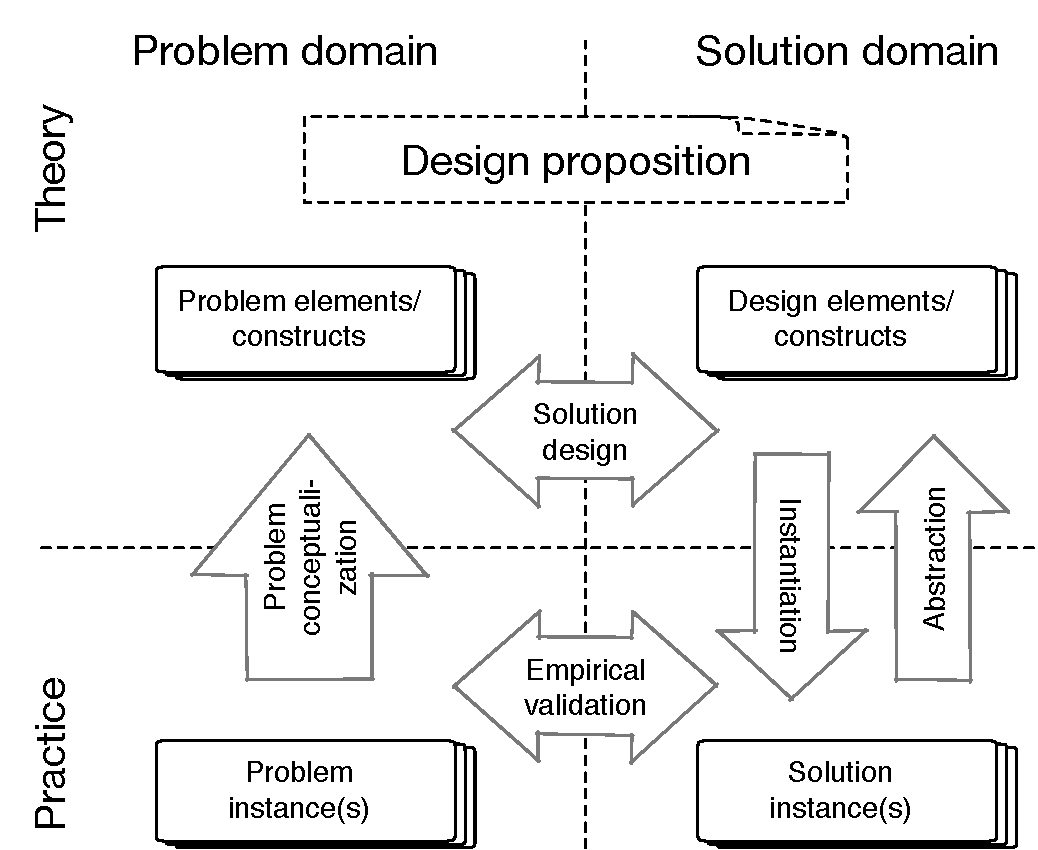
\includegraphics[width=0.8\textwidth]{Figures/DS_model.pdf}
% figure caption is below the figure
\caption{Model of design science contributions in software engineering~\cite{Engstrom19arxiv}. The boxes represents theoretical and practical contributions of design science research and the arrows represent knowledge creating activities that can be performed by both practitioners and researchers.}
\label{fig:DS_model}       % Give a unique label
\end{figure}



\subsection{Technological rules}
\label{sec:technologicalrules}



% outline: The technological rule is the theoretical contribution of design science research also referred to as design knowledge.
The technological rule captures generalized knowledge about mappings between instances of problems and solutions (i.e. in-context validations) and is thus a means to transfer knowledge between contexts. The technological rule spans both a problem domain and a solution domain and is formulated based on constructs in both domains. 

\per{Emelie - check changes.}
In a technological rule the solution (or intervention) may refer to the use of a specific tool or the application of a more general approach. The scope of validity of the solution is described in terms of a desired effect in a situation.  Wieringa refers to this as \emph{design theory}, defining it as theories of artifacts in context~\cite{wieringa_design_2009}. The design knowledge within the technological rule aims to help software engineering professionals design customized solutions to their specific problems. Ideally it is a general recommendation based on current state of art including the new additional contribution of a piece of research.

% outline: It can typically be expressed as: 'To achieve <desired effect> in <context> apply <intervention>
Technological rules comprise both the context in terms of the \emph{desired effect} and \emph{the situation}, and a prescription in terms of a \emph{proposed intervention}. Thereby it frames the research outcome in terms of desired effects and interventions rather than in terms of a solution to a problem. The term \emph{technological rule} originates from Bunge~\cite{bunge_philosophy_1998} and corresponds to \emph{design theories} in Gregor and Hevner's work~\cite{gregor_positioning_2013}. %Our visual abstract template,  see Figure~\ref{fig:VA-template}, emphasizes technological rules as the main takeaway of design science within software engineering research. 
A technological rule can typically be expressed in the form: 

\begin{center}{\emph{To achieve \textless Effect \textgreater ~ in \textless Situation \textgreater~apply \textless Intervention\textgreater}.} 
%\newline
\end{center}

Here, a class of software engineering problems are generalized to a stakeholder's desired effect of applying a potential intervention in a specified situation. 
Making this problem generalization explicit helps the researcher identify and communicate the different value-creating aspects of a research study or program.



% outline: The abstraction level may vary
Wieringa and Daneva address generalisability of design theory~\cite{wieringa_six_2015} and argue that there is no such thing as general design theories. Instead they emphasise the utility of \emph{middle-ranged theory}, defined as theories lacking universal scope. 
Technological rules are examples of such middle-ranged theories that can be expressed at any convenient abstraction level. However, technological rules expressed at a very high abstraction level (e.g. ``To produce software of high quality apply good software engineering practices'') tend to be either trivial or too bold (easy to debunk) while rules at very low abstraction levels have a narrow scope and thus lack relevance for most software engineers. 

How the intervention in a technological rule is formulated may vary. It could, for example, refer to the use of a tool or articulate abstractions of the knowledge embedded in the tool. It could also refer to the application of a practice, a technique, a framework or a set of guidelines. Examples of technological rules were extracted from a set of distinguished ICSE-papers from 2014--2018~\cite{Engstrom19arxiv}. These are available online at dsse.org.

One single instance of a problem-solution pair can generate multiple technological rules that are hierarchically related to each other. \per{Add example?}Similarly there are hierarchical relationships with prior related technological rules to which a specific contribution is compared.
Thus it is important to explicitly formulate the technological rule when presenting design science research and to be consistent with it both when arguing for its relevance and its novelty as well as when presenting the empirical (or analytical) support for the claims.  A research contribution may refine any of the three constituents of an existing rule, add empirical support for the rule as a whole or propose a new rule.

% outline: Technological rules are validated by in-context validations (investigations of instantiations of the rule)


\subsection{Problem and design constructs}
\label{sec:constructs}
Another type of theoretical knowledge, produced in design science is the 
constructs on which we build technological rules, that is, the conceptualization of the problem domain and the solution domain, respectively.  
A construct can for example be a taxonomy that is used to articulate a technological rule or to classify a set of technological rules in a research review. Taxonomies provide means to relate different technological rules to each other. The different constituents of a technological rule may belong to different taxonomies. A construct can also be a conceptual model or a conceptualization approach that helps describing a problem in terms of an envisioned solution

Design knowledge is gained by investigating one or more instances of a solution in context~\cite{wieringa_what_2014}. Each instantiation (for example, a case study or an iteration of action research) constitutes a unit of analysis in relation to the technological rule and the new knowledge is communicated and assessed from that perspective. 

\subsection{Problem characterization and solution design}

 % Who, What, Where, When, Why and How

% (Who?) Problem understanding is ultimately an act of the practitioner but could be done in collaboration between researchers and practitioners or by researchers alone

In the long run, software engineering theory aims at helping practitioners designing solutions to their specific problem. Thus problem understanding is ideally an act of a software engineering practitioner and not a researcher. However, to produce such theory, research is needed. In the previous section we describe how design knowledge is obtained and matures through observations of real life instances of problem-solution pairs. For each such instance the problem needs to be formulated (understood) according to a conceptual lens. Such problem understanding can take place in collaboration between practitioners and researchers in, for example, action research or case study research, or by researchers observing software engineering practice.

% (What?) The outcome of the problem understanding step is a conceptualuzation of the problem instance towards an envisioned solution and thus tightly connected to a specific design approach

The outcome of the problem understanding activities is a conceptualization of the problem instance towards an envisioned solution. If, for example, the proposed solution is to design a visualisation system, the problem should typically be described in terms of a group of target users, their questions and tasks, and their measurements or data~\cite{meyer_nested_2015}. Thus the problem formulation is tightly connected to the solution design and cannot be done in isolation. The problem understanding is to a large extent in the eye of the beholder. A behavioral scientist would, for example,  make a different problem description of a software project, compared to a software engineering researcher, and different software engineering researchers are influence by their background as well. This implies that the problem understanding is intertwined with the solution design.

Although we consider much of the software engineering research to be design science research, not all exploratory and descriptive research provide design knowledge. The combination of problem understanding with the envisioned solution makes it design science.

% (What?) The research contribution is not the conceptualization, but the identification of the problem instance (empirical support for prevalence of a conceptual problem) and potential updates of the modelling approach (new aspects of the technological rule)

Furthermore, the research contribution is \emph{not} the conceptualization as such, since this is connected to the instance of the problem and not the class of problems. Instead the research contribution is the empirical support for new, existing or refined technological rules. A research contribution from the problem understanding step could for example be the identification of problem instances -- confirming the prevalence of a general problem -- or updates of the conceptualization approach -- i.e. the design constructs of a general solution.

% (When?) Problem understanding is the first step towards a solution design.

Problem understanding is the first step towards a solution design. However, depending on the type of solution, problem understanding may need to be repeated at several abstraction levels starting with the stakeholder's problem description and, for example, in case of a tool implementation reaching to the level of implementation details (such as  choice of algorithm). If this is the case, different types of technological rules are used and validated at different abstraction levels. It is important to be aware of which these rules are and ensure that the validation of a solution takes place at all these levels and that the validations are mapped to the correct technological rules. 

% (Where?) Problem understanding must originate in empirical observations of practice
Software engineering is a discipline, in which conditions are rapidly changing. To provide relevant recommendations -- technological rules -- problem understanding must originate in empirical observations of practice, i.e. real life problem instances. Furthermore, software engineering is a socio-technical endeavor implying that stakeholders need to be involved in both problem understanding and solution validation, at least for technological rules at the higher abstraction levels. Lower level technological rules may be investigated in isolation but must be related to the higher level rules to be of relevance. 
% (How?) Problem understanding should build on prior work
Ideally problem understanding can be guided by theory, i.e. prior technological rules and conceptualization approaches. 



%\subsection{Solution design}


%Solution design is one out of three knowledgecreating activities in the software engineering design cycle
%Design science comprises both creation and validation of design knowledge, i.e. prescriptive and context dependant knowledge. Such knowledge can be achieved by investigating real world instances of problem-solution pairs. We have identified three different knowledge creating activities of which the \emph{solution design} is one. The other two are the \emph{problem understanding} and the \emph{empirical validation} of the solution to the problem in context, see Figure~\ref{fig:VA-template}


%Ultimately an act of a SE practitioner
Just like problem understanding, the actual design of a real-life solution is the act of the practitioner, preferably guided by design knowledge produced by researchers. %Building on previous work/technological rule
Guided by existing technological rules, see Section~\ref{sec:technologicalrules}, and related research outputs, a practitioner should be able to identify and adopt possible solutions to their context. However, one activity in the production of design knowledge is to work through increments of a solution design, either together with practitioners in a real-life setting or off-line. %Creative process/alternative solutions should be considered/design decisions reported
While the solution design is a creative activity, the design knowledge it produces can be made more accessible and trustworthy if critical design decisions are clearly reported together with considerations about alternative solutions.



%May include several levels of design/evaluation and validation 


%Reflections on the design process less important in the SE domain than in the IS domain
Wieringa describes design science as an act of producing knowledge by designing useful things~\cite{wieringa_design_2009} and makes a distinction between \emph{knowledge} problems and \emph{practical} problems. Similarily, Gregor and Hevner emphasise the dual focus on the artifact and its design in information systems~\cite{gregor_positioning_2013}, and argue for an iterative design process where validation of the artifact provides feedback information to improve both the design process and the artifact. Although such an approach may be relevant for designing software engineering artifacts too, there is an important difference between the two research domains: while information systems refers to a solution domain, software engineering research originates in a problem domain with a plethora of more or less sophisticated solutions, not necessarily artifacts. Thus the empirical contribution to problem understanding is of higher importance in the software engineering context while the reflection on the design as such is of less value compared to research contributions in a typical solution domain such as information systems. Still, in both cases it is design knowledge that is produced as the aim is to produce prescriptive knowledge for practitioners in their respective domain. 

 

\subsection{Validation, instantiation and abstraction}

To validate a technological rule it must be instantiated, preferable in multiple cases of problem solution-pairs instantiating the rule. Each such case adds to the strength of validity of the rule. The other way around is also possible, i.e. that a new technological rule may be abstracted from an observed implemented solution to a real life problem.

Validation of research under the design science paradigm is always about a problem--solution pair in \emph{context}. The constituents of the technological rule implicitly specify the validation activities; the \emph{intervention} is the object of study, the \emph{situation} defines the context, and the expected \emph{effect} defines the validation criteria. This points to the `in vivo' software engineering context as the ultimate validation context for design science research. Multiple case studies are consequently brought forward as the natural research methodology in design science \cite{van_aken_management_2004}. However, for some design problems, the characteristics of the context may be resembled in `in vitro' settings for the validation. For example, a tool which has no human--tool interaction can be evaluated with real or realistic data in an off-line setting. In other cases, practical och economical limitations can prevent the research endeavor from taking place in real, operational environments, and thus scaled down validation contexts may be used in the research. 
The risks related to validating interventions in business critical contexts may be high. If the intervention does not deliver the effect as expected, the outcome of the software engineering activity as a whole may be endangered. Further, the costs related to implementing the intervention may also be high -- for example changing a work flow or adapting the information infrastructure to a new tool. Thus, validation procedures may be used, which gradually extend the validation scope for the intervention.

On the other hand, reducing the scope and complexity of the validation context too much may take away the realism which is essential for addressing a relevant problem with a feasible solution. `In vitro' studies may be useful to validate specific mechanisms, but they are not feasible for complex systems studies.  

Stol and Fitzgerald adapted Runkel and McGrath's framework for research strategies, to guide balancing generalizability, precision and realism in designing validation studies \cite{StolABC18}. This framework may be useful in choosing research strategies in relation to the goals of the research endeavor. The framework defines two dimensions of i) universality/specificity of context and systems, and ii) level of obtrusiveness. Maximum potential realism is achieved with specific contexts and systems, and more or less obtrusive research, depending on the perspective of explanatory research (field study) or design science (field experiments).  

The specific choice of methods for the validation depends on the research question. Easterbrook \emph{et al.} provide guidance to the selection of methods and conclude for the philosophical stand behind design science: ``Pragmatists use any available methods, and strongly prefer mixed methods research, where several methods are used to shed light on the issue under study''~\cite{easterbrook_selecting_2008}. This recommendation fits well with the design science paradigm and its pragmatists viewpoint.

Furthermore, the choice of method depends on the abstraction level of the validation. Munzner illustrate this in a nested model for visualisation design and validation, see Figure~\ref{fig:nested_model}. This model illustrates how one design science project must respond to validity questions at several levels of abstraction, and that it is important to be consistent when selecting validation method to avoid mismatching between levels. As discussed in Section~\ref{sec:technologicalrules}, technological rules may be defined at all these different levels and the scope of validity of each rule is defined by the context in terms of the conceptualization of the problem at the current abstraction level.

\begin{figure}[t]
  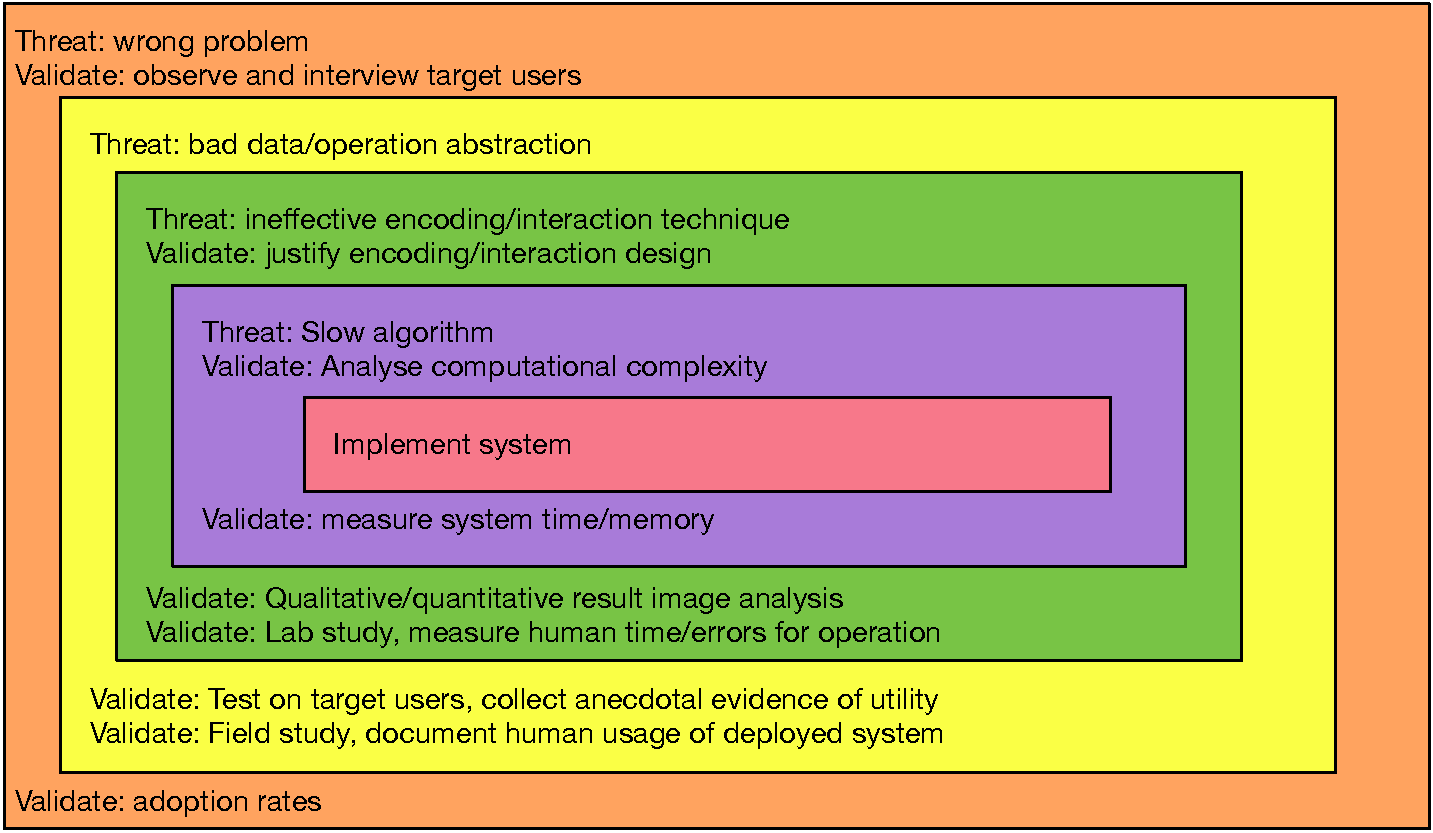
\includegraphics[width=0.9\textwidth]{Figures/nested_model.pdf}
% figure caption is below the figure
\caption{Nested model for vizualisation design and validation~\cite{munzner2009}.}
\label{fig:nested_model}       % Give a unique label
\end{figure} 

The design science paradigm builds primarily on theoretical/analytical generalization, in contrast to explanatory sciences, which mostly rely on statistical generalization~\cite[p. 30]{Runeson12Case}. Extending the scope of validity for a technological rule, i.e. creating a new more general rule, is done by applying the intervention to new contexts or by reasoning about the validity to another context, by comparing key characteristics of the contexts. This is referred to as case-based generalization~\cite{wieringa_six_2015}.  

Technological rules may also develop from the general to the specific. The research may starts with a general rule which is refined as new knowledge is gained through the instantiation of the rule in multiple contexts. 


\subsection{Research Methods in Design Science} 


Design science may embrace a multitude of research methods to be used. For the \emph{problem understanding} and \emph{validation} of technological rules, empirical research methods are used. Methods supporting realism and natural settings~\cite{StolABC18} are preferred as the problem in context is in focus for design science research. 

As mentioned above, the typical research methodology used to study and test technological rules is multiple case studies. In the case studies, a series of problems of the same class is adressed. Design knowledge is built up through the empirical validation of the solution in context. Case study methodology is well established in software engineering \cite{Runeson12Case} and fits thus well into the design science paradigm. In a survey of 101 industry-academia collaboration projects, Garousi \emph{et al.} found 75 that were characterized as case studies~\cite{Garousi2019}. Further, they note that ``industrial case studies usually apply either the `exploratory' or the `improving' type, or both, rather than other case study types (descriptive, explanatory)''. Methods for data collection and analysis can be selected from the rich plethora of options available for such studies, for example, interviews, focus groups, observational studies, archival data, and software metrics. 

Action research is another way of producing and validating technological rules, as indicated by 41 out of the 101 industry-academia collaboration projects surveyed by Garousi \emph{et al.} were labeled as action research \cite{Garousi2019}. However action research does not explicitly aim at developing knowledge that can be transferred to other contexts but rather to make a change in one specific local context. Both Wieringa~\cite{wieringa_technical_2012} and Johannesson~\cite{johannesson_introduction_2014} discuss action research as one of several empirical methods that can be used to produce design knowledge.


\begin{figure}[t]
  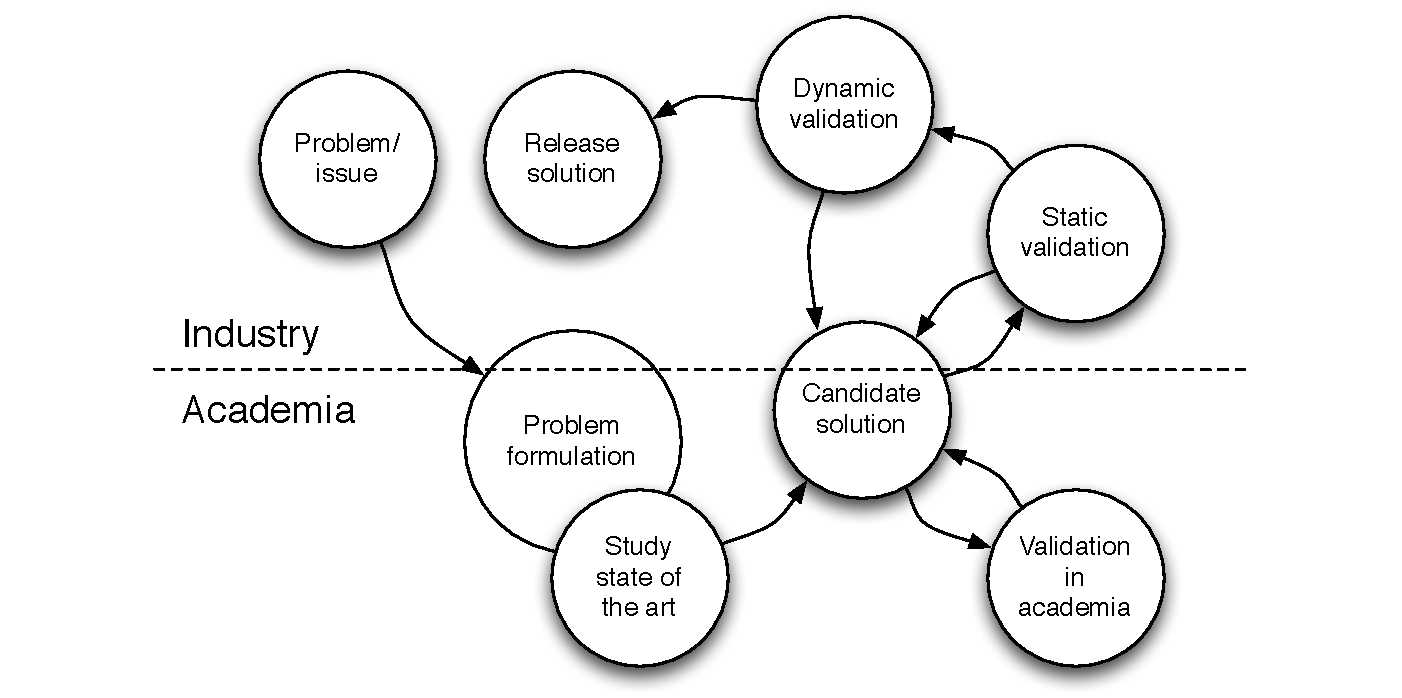
\includegraphics[width=0.9\textwidth]{Figures/GorschekModel.pdf}
% figure caption is below the figure
\caption{Model for technology transfer in practice' \cite{GorschekSW2006}.}
\label{fig:GorschekModel}       % Give a unique label
\end{figure}

Gorschek \emph{et al.} defined a ``model for technology transfer in practice'' \cite{GorschekSW2006} focussing on industry--academia collaboration, which has some elements of design science, see Figure \ref{fig:GorschekModel}. The model, which prescribes conceptual steps in solving a problem in an industry-academia collaboration setting, has elements of problem identification and formulation. The design of solutions involve studying the literature (state of the art) and selection of a candidate solution. This solution is validated in three steps, in academia, statically, and dynamically, before it is released into operations. 

All these elements fit into the design science lens, although the model (by intention) focuses primarily on the artifact and specific context, rather than the generalized knowledge and technological rule, which are significant element of design science research. Further, when taking the generalization of knowledge and iterative knowledge building is stressed, it becomes clear that industry--academia collaboration is not a one-way transfer of technology, but a mutual interaction between the two.


\section{Using the Design Science Frame in Software Engineering}
\label{sec:UsingDSinSE}


In this chapter, we focus on how the design science paradigm can be used as a frame for software engineering research. Software engineering research aims at improving practice, which implies needs for various kinds of collaboration between researchers and practitioners. In their practitioner article on industry--academia collaboration in software engineering, Carver and Prikladnicki stress the importance of a synergistic relationship between software practitioners and software engineering researchers.
\begin{quote}Practitioners could obtain more relevant research results, and researchers could better understand the type and scope of problems to examine.~\cite{CarverIEEESW2018}
\end{quote} 

These practitioner--researcher synergies resonate well with the design science paradigm.  We use a \emph{visual abstract template} as a tool to analyze design science constructs in software engineering research (Section~\ref{sec:VA_template}). We suggest three direct uses of the design science paradigm as a frame for software engineering research, which we illustrate through \per{an example/two examples}(Section~\ref{sec:examples}). Firstly, it can help in assessing contributions in research, both for the research community and during the planning and design of a research project (Section~\ref{sec:assessment}). Secondly, design science, particularly the technological rule, can be used in knowledge building, synthesizing and advancing the theoretical knowledge in the software engineering field (Section~\ref{sec:knowledge}). Thirdly, the design science frame may help in communicating research across the community and with industry (Section~\ref{sec:communication}). 


\subsection{A template to highlight design science constructs in software engineering}
\label{sec:VA_template}

%Design Science Studie

\begin{figure}[t]
% Use the relevant command to insert your figure file.
% For example, with the graphicx package use
  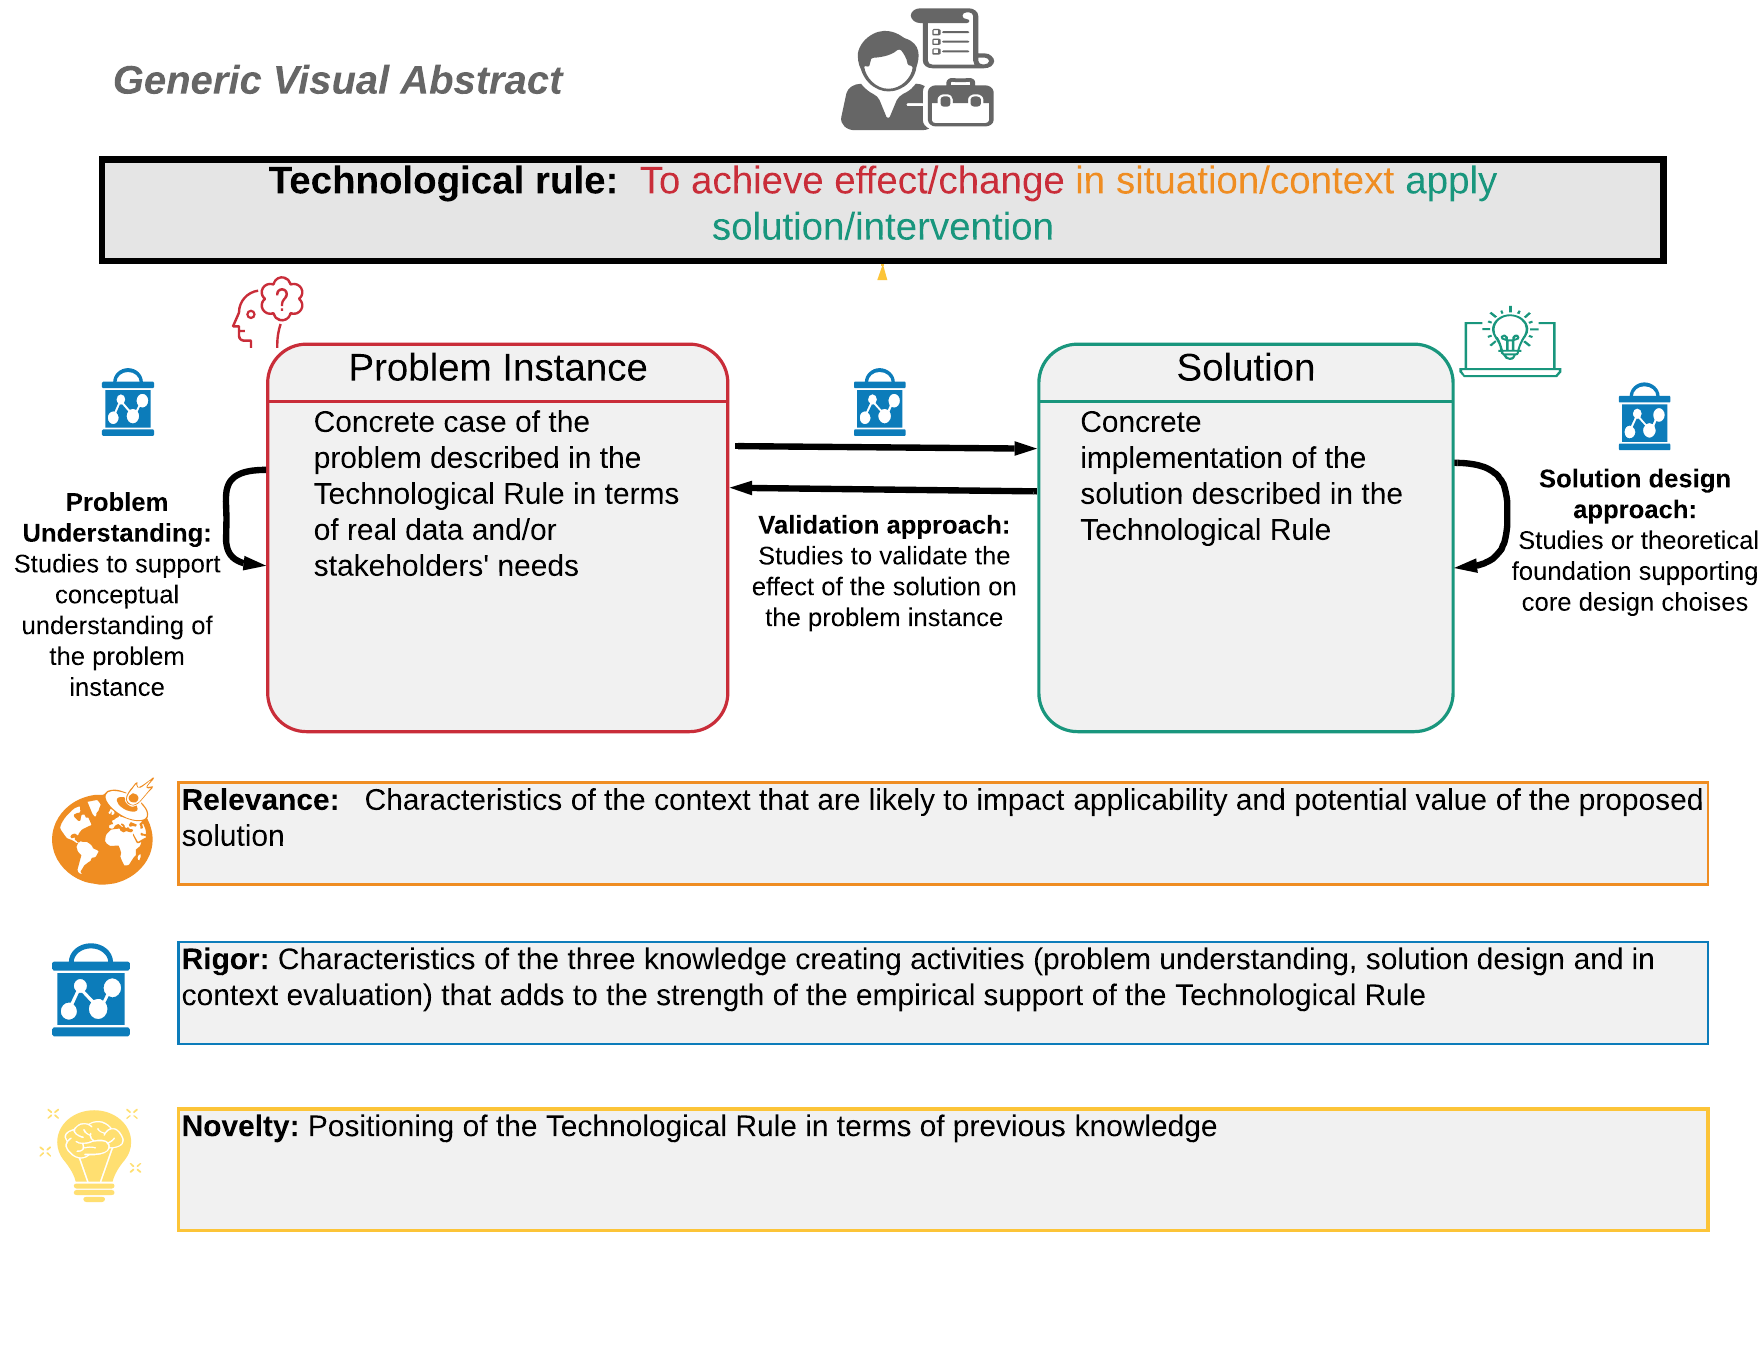
\includegraphics[width=1.0\textwidth]{Figures/GenericVA.png}
% figure caption is below the figure
\caption{Visual abstract template including the core constructs in the design science paradigm.}
\label{fig:VA-template}       % Give a unique label
\end{figure}


%Design Science as a Lens
In an analysis of software engineering research, we concluded that the design science perspective fits well with the field, the design science perspective is rarely used explicitly to design and present software engineering research. We therefore designed a \emph{visual abstract template} to help identifying the design science constructs in software engineering research \cite{StoreyESEM17}, see Figure~\ref{fig:VA-template}. We further extended the template with survey questions, to help analyze software engineering literature from a design science perspective \cite{Engstrom19arxiv}. The template aims to capture the key takeaway from a research study to help researchers assess the research contribution, build knowledge iteratively, and communicate research to practitioners. %Note connections to end of this chapter

Our design science template covers the main constructs of design science research: The theoretical contribution in terms of a \emph{technological rule}; its instantiation in terms of a real \emph{problem--solution} pair;  the empirical or theoretical support for the \emph{problem} understanding, the \emph{solution} design. Further, the bottom three boxes address the \emph{relevance} of the research, the \emph{rigor} of the research activities,  and a statement about what makes the technological rule \emph{novel} in relation to the underpinning research, be it with focus on a refined problem conceptualization a new or improved solution design, or a validation of the the technological rule in a new context. 




\subsection{Design Science Example}
\label{sec:examples}
To illustrate the use of the design science lens for software engineering research, we present and discuss an example by Jonsson \emph{et al.}, introducing automated bug assignment to handle a large inflow of bug reports \cite{JonssonBug15}. We have used the same example to illustrate our visual abstract \cite{StoreyESEM17}, see Figure \ref{fig:BugAssignment}.

\begin{figure*}[t]
\begin{center}
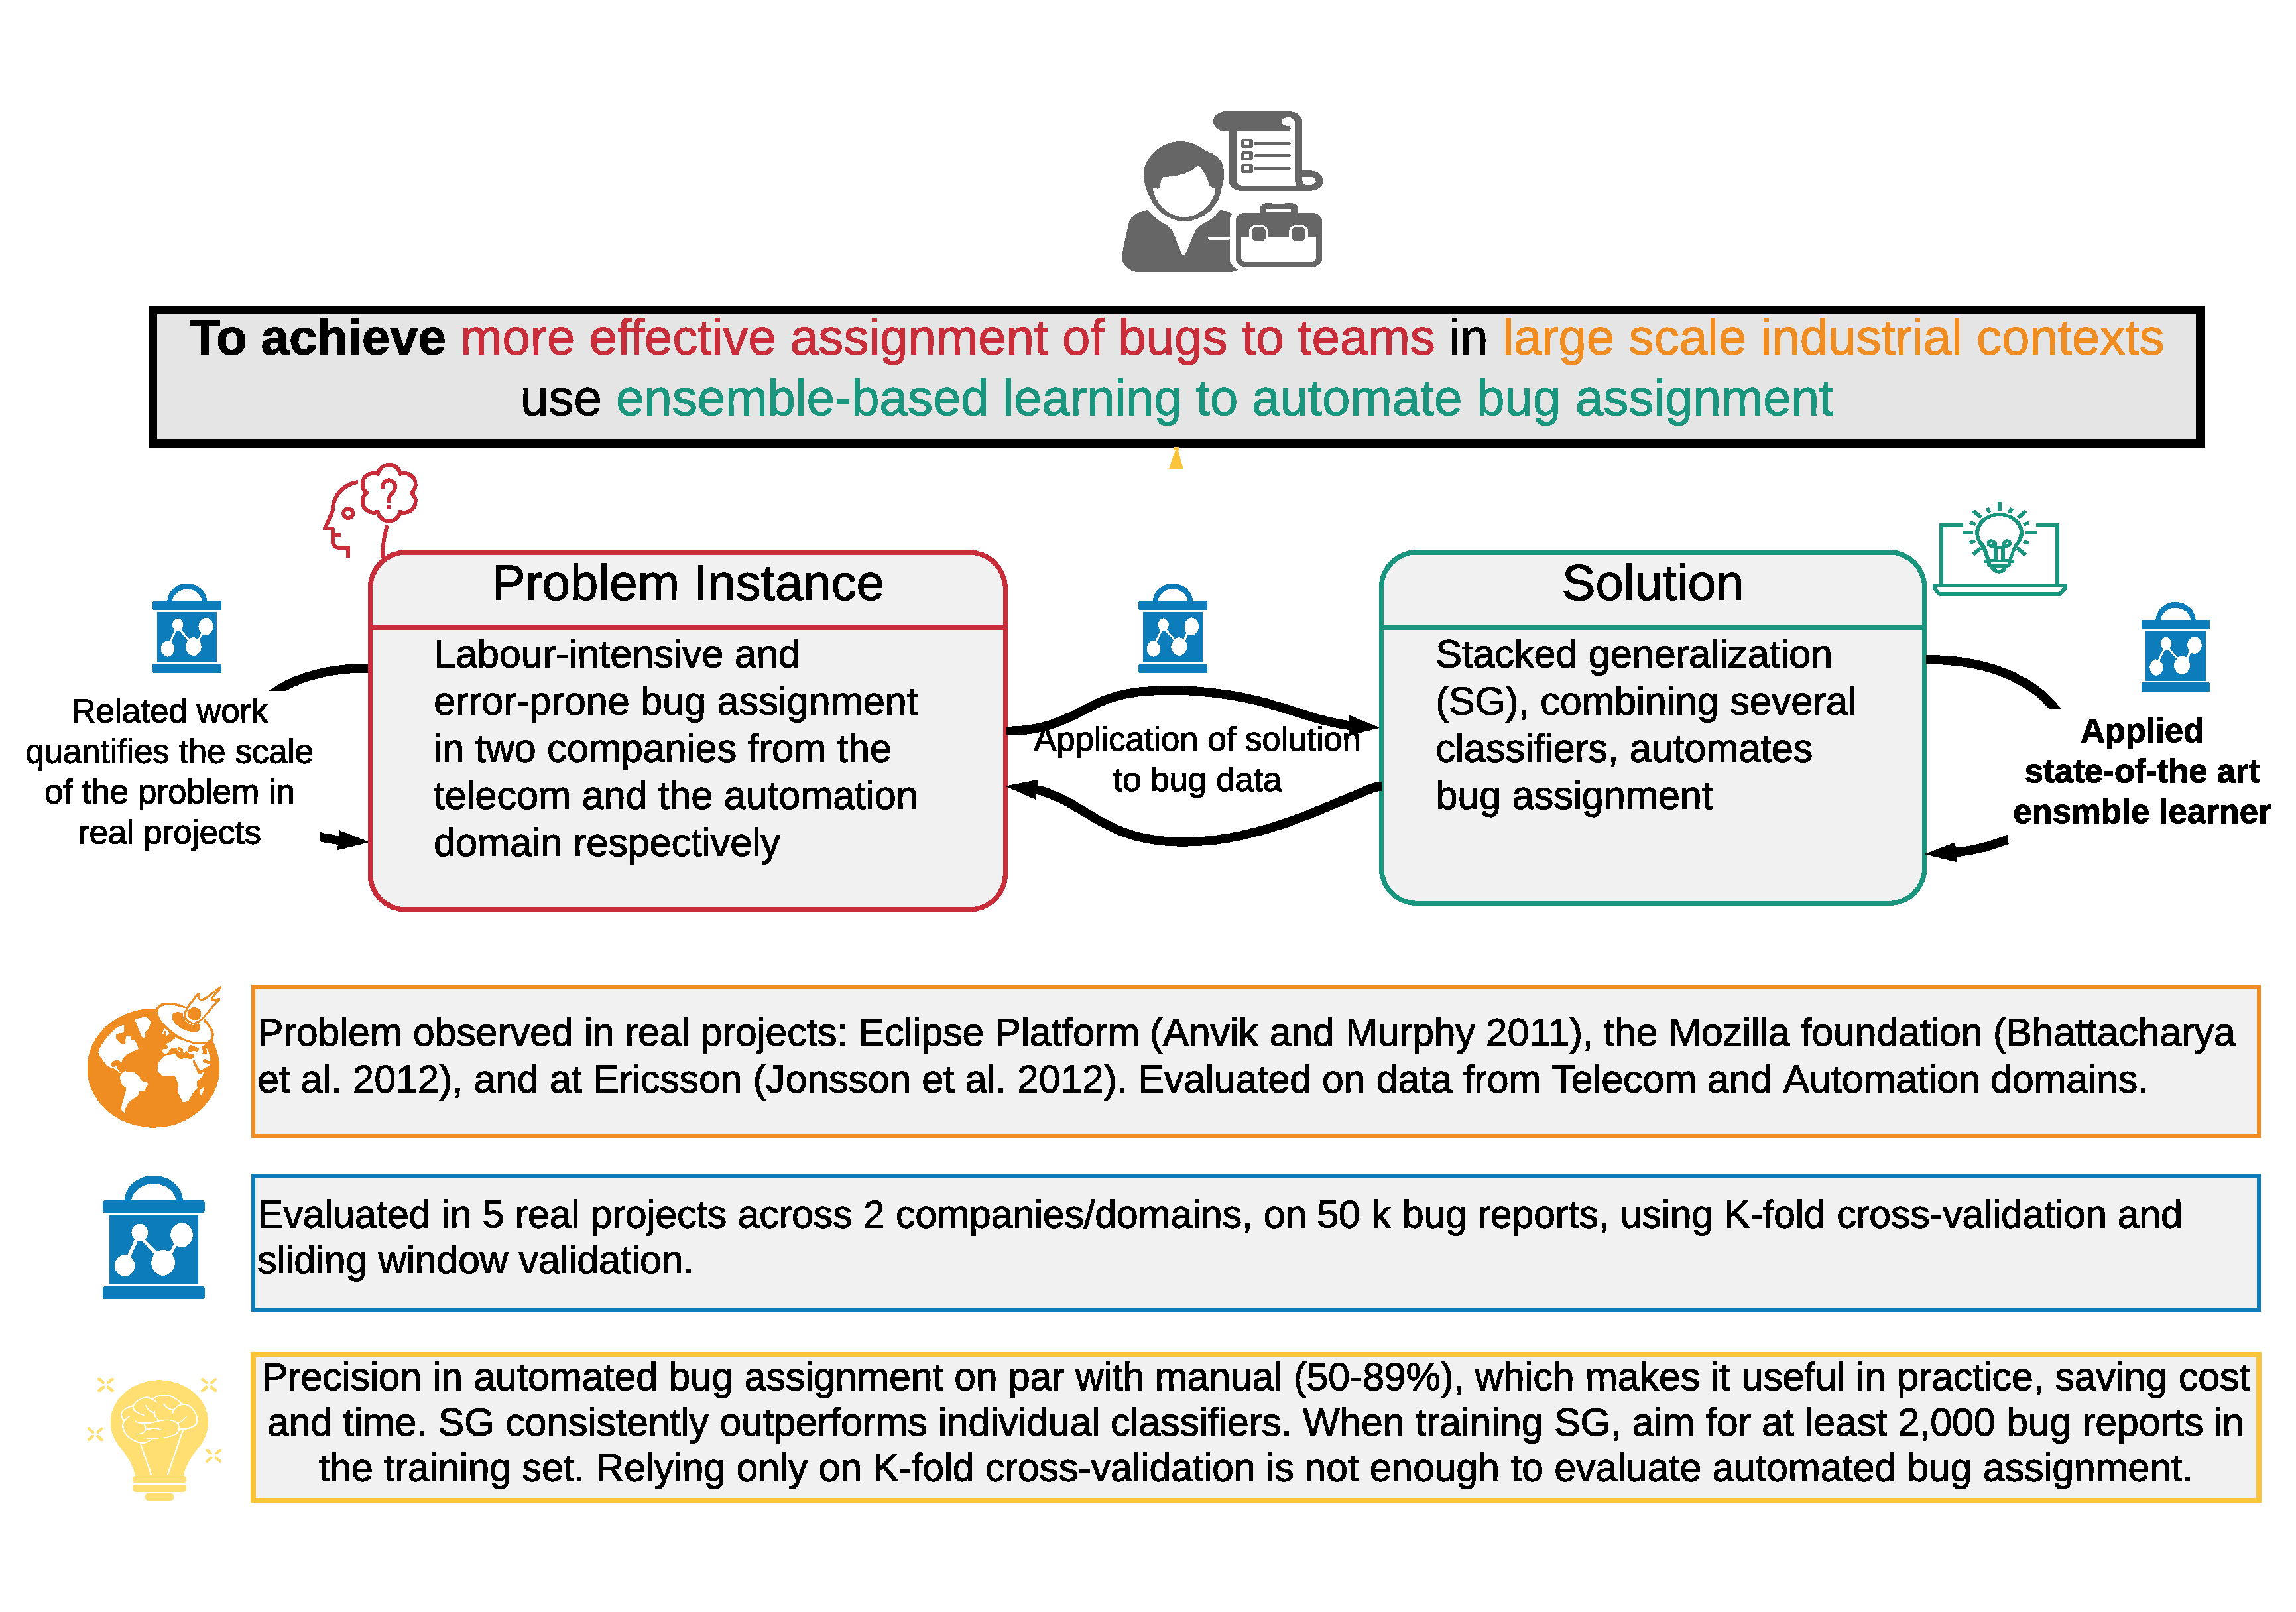
\includegraphics[width=\columnwidth, trim={5mm 20mm 5mm 20mm },clip]{Figures/VATemplateJonsson.pdf}
\caption{Visual abstract for the paper on automated bug assignment \cite{JonssonBug15}.}
\label{fig:BugAssignment}
\end{center}
\end{figure*}

The automated bug assignment research was not originally presented through the design science lens. However, like much software engineering research it is implicitly conducted as design science research \cite{Engstrom19arxiv}. 
The scientific knowledge gained from the work can be phrased as a \emph{technological rule}:
\begin{quote}{To achieve more effective assignment of bugs to teams in large scale industrial contexts use ensemble-based machine learning to automate bug assignment. \cite{StoreyESEM17}}\end{quote}

The general \emph{problem} on inefficient bug assignment is observed in the literature as well as in the specific industrial contexts, where this research was conducted. With a solution in mind to use machine learning techniques to assign bugs to teams, the characteristics of the defect data and the organizational context were explored. We thus identified the characteristics of the \emph{problem instance}. Related work on bug classification, as well as on machine learning techniques, underpinned the \emph{design decisions} for the proposed solution. The machine learning solutions were implemented in the Weka framework \cite{hall_weka_2009}, and trained and several alternative solution instances were \emph{validated} on real data from five projects across two companies/domains, on 50~000 bug reports. For the specific companies, a design artifact was produced, namely the bug assignment tool built on top of Weka.

The \emph{relevance} of the research is ensured by being anchored in the literature as well as in the specific problem instances of the study. Research \emph{rigor} is ensured by structured and transparent research methods, conducted with real world data. The \emph{novelty} of the research lies in the technological rule, embedding the choice of machine learning classifiers (ensemble-based), validating the ability to demonstrate a system of automated bug assignment which precision is on par with the existing manual procedures.

Our example study of automated bug assignment was conducted in several steps, which can be described in terms of the technology transfer model in Figure \ref{fig:GorschekModel}:
\begin{itemize}
\item \emph{Problem/issue}: Overall problem phrased as manual assignment of bugs to teams being costly and error prone
\item \emph{Problem formulation}: Indepth studies of defect reports and their links to other information elements and activities helped characterize the problem
\item \emph{Study state of the art}: A systematic mapping study was performed of trace-link research, identifying the theoretical foundation \cite{Borg2013EMSE}
\item \emph{Candidate solution}: Development of experimental tools, supporting multiple algorithms
\item \emph{Validation in academia}: Comparison of algorithm performance in academic research \cite{BorgESEM13}
\item \emph{Dynamic validation}: Training and cross-validation of tool on real data sets \cite{JonssonBug15}
\item \emph{Release solution}: Incorporation of a simplified version of the tools in to the company's toolset
\end{itemize} 

In this case, we performed no static validation as we had the opportunity to make a dynamic off-line validation with real industry data. We use the example below when discussing the use of the design science as a fram to assess research contributions, build knowledge, and communicate research.



\subsection{Assessment of contributions}
\label{sec:assessment}

Assessment of research contributions can be conducted proactively (when relevance may be a primary concern for consideration before the research is executed), prospectively (as the research is ongoing and when rigor should be carefully considered), or retrospectively (where novelty of the design knowledge produced may become more evident).
Below, we discuss assessments of contributions and refer to the examples above.



% Peggy:  not sure what to do with this...
%\paragraph{Validation should be made in context and test the impact of the solution on the real problem}

\subsubsection{Relevance %of a design science study is described in terms of problem similarity and solution applicability.
} 

Relevance of a design science study is described in terms of problem similarity and solution applicability. The relevance of a research contribution could be viewed from two perspectives: from the perspective of other practitioners that may benefit from the design knowledge produced and from the perspective of the research community. 

From an individual practitioner's point of view, the relevance of a research contribution may be assessed by comparing their specific context with the study context described in the research report. 
A practitioner may need to consider their specific context may allow the design knowledge to applied as is, or if it should be customized in some way, or perhaps the knowledge may not apply at all to their situation or problem.
%In the example by Shi \emph{et al.}, (see Fig.~\ref{fig:VA-example}) a practitioner may similarly face the challenge of testing very larger systems and  that they too could benefit from using historical build information and test dependencies to guide which tests should be run (or not).
In the example by Jonsson \emph{et al.}, (see Figure \ref{fig:BugAssignment}) a practitioner may  similarly face the challenge of manually assigning bugs to teams and  that they too could benefit from using ensemble-based machine learning to automate the bug assignment (or not).

From the research community perspective, relevance is often considered in terms of how common the studied problem is and how generalizable the produced design knowledge may be. To enable both types of assessments, relevant context factors need to be reported. Not all context factors are helpful in making this assessment but only those that are critical for either the applicability of the solution or for the potential gain of applying the solution. 
%Referring to the example by Shi \emph{et al.}, reducing wasteful test executions is a frequent topic of research in software engineering and builds on much evidence that this problem is also relevant in practice.
Referring to the example by Jonsson \emph{et al.}, applying machine learning to bud assignment is  a frequent topic of research in software engineering. They report 20 previous studies on machine-learning based bug assignment \cite[Fig.2]{JonssonBug15}, and also adds evidence that this problem is relevant in practice.

\subsubsection{Rigor %of a design science study refers to the strength of the added support for the technological rule.
} 
Rigor of a design science study refers to the strength of the added support for the technological rule. It may be assessed in all of the three knowledge creating activities (problem understanding, design and solution validation). 
Rigor should be considered when the research project is designed, as well as throughout the project and afterwards to reflect on possible threats to validity. 

It is worth noting that the solution design activity is by nature a creative process and does not necessarily have to add to the rigor of the research overall. One aspect of rigor in the design activity could be the extent to which a solution is built on prior design knowledge, and in such cases consideration of alternative solutions can be taken in to account. 
In the case by Jonsson \emph{et al.} they choose alternative classifiers from the Weka tool by reasoning about their properties, and combined them into ensembles of classifiers for evaluation.
%Alternative, rigor in the problem understanding phase (which is the case of the research by Shi \emph{et al.}) can be used to guide a solution design which is what happened in the case of the research by Shi \emph{et al.} as their mathematical formulation of wasteful test executions guided them towards the solution to consider test movements based on historical build information and actual dependencies of tests. 

The other two activities, i.e. problem understanding and solution validation, are on the other hand based on common empirical methods on which relevant validity criteria can be applied. For example, the study by Jonsson \emph{et al.} can be considered high in rigor as the proposed solution is validated by its application to 5 defect datasets from two large software systems, comprising 50~000 bugs.  Furthermore, they found that the precision in the automated bug assignment was on par with the manual industry practice, which makes it useful in practice.
%For example, the study by Shi \emph{et al.} can be considered high in rigor as the proposed solution is validated by its application to 5 large software systems.  Furthermore, they found that developers accepted 84\% of the recommendations made by their proposed intervention (the TestOptimizer tool). 

\subsubsection{Novelty %of a design science study is expressed in terms of new or refined technological rules.
} 
Novelty of a design science study is expressed in terms of new or refined technological rules. Technological rules may be expressed at several abstraction levels, thus it is always possible to identify an abstraction level at which a research contribution is novel, may it be at the cost of general relevance.  In the research by Jonsson \emph{et al.}, novelty of the intervention proposed in the technological rule is not straightforward to assess, as there already existed 20 studies on machine-learning to automate bug assignment. The novel contribution here is the systematic design and evaluation of a machine learning approach, applied to a real-world context, as expressed in the technological rule.
%In the research by Shi \emph{et al.}, novelty of the intervention proposed in the technological rule is rather easy to assess, as the TestOptimizer tool (and the techniques it embodies) is a novel contribution.  

However, novelty may not always be a priority in a given research effort.
To optimize rigor, novelty and relevance of reported research, the researchers should strive to express the technological rule at the highest possible abstraction level, at which it is novel, the provided evidence give strong support and are not debunked by previous studies (or common sense). However, adding empirical support for existing, but under-validated, technological rules have a value of its own, which makes novelty less important than the rigor and relevance criteria.


\subsection{Knowledge building}
\label{sec:knowledge}

Articulating the knowledge that is produced by our research in a more uniform way may help in building and synthesizing related knowledge in our community. 
The technological rules that emerge can at best be considered as theory fragments that prescribe and predict how a certain intervention for a particular context will lead to a proposed change. 
But our hope is that linking technological rules that are related (perhaps in hierarchical form) may over time help our community arrive at theories that may be more general, and that can be refined and improved over time. 

%For example, Shi \emph{et al.}'s research on reducing wasteful text executions can be related to other test minimization technological rules which together may be more generalizable. 
For example, Jonsson \emph{et al.}'s research on automated bug assignment is related to previous bug assignment research, although it is hard to compare due to lack of detail and non-standardized validation practice. If the contributions were clearly expressed as technological rules with corresponding validation, the outcomes together would be more generalizable. 

\subsection{Research communication}
\label{sec:communication}

As we discussed above, building design knowledge in software engineering requires a close partnership and relies on tight collaborations with practitioners. 
Practitioners play a participatory role in our research by confirming and eliciting problems to be solved, as well as by designing practical solutions using design knowledge, and then validating them in context (on real problem instances). 
Consequently, how we communicate our research to practitioners is critical to this participatory research approach. 

We feel the technological rules will be valuable in communicating our findings to industry and that the visual abstract may also appeal to some practitioners wanting to quickly gain a bigger picture of the research that is behind the design knowledge embodied by the technological rule. 
We are currently in the process of getting feedback from industry partners.  For example, see \url{http://dsse.org} for a collection of visual abstracts we authored based on the distinguished papers from ICSE from 2014 to 2018.  

Other examples include Petersen and Engstr\"om's framework, SERP taxonomy architecture~\cite{petersen_finding_2014} including the constructs of a technological rule  
(i.e. desired effect, context and intervention), to support the mapping of practical problems with research. 
This framework has then been used to develop a taxonomy to establish a common understanding between practitioners and researchers in software testing~\cite{engstrom_SERP-test_2017} and to review regression testing literature from a relevance point of view~\cite{ali_search_2019}, leading to generalized recommendations in terms of technological rules. 

Another attempt to make evidence available to practitioners is presented by Cartaxo et al. \cite{Cartaxo2016}. 
They present the concept of ``evidence briefings'', which is a way to summarize Systematic Literature Reviews in a one-page format. 
They used accepted information design principles to design the structure of the one-page briefing. The format and content were positively validated the by both practitioners and researchers. While evidence briefings may provide an effective way to synthesize evidence from several studies our visual abstract template provides a means to effectively summarize the contribution of one study or research program from a design science perspective.

%\section{Examples}
%Either we choose examples that illustrate the different aspects of DS, or we choose three examples that are good examples of DS -- candidates from the ICSE best papers, or our own papers?


\section{Recommended Further Reading}
\label{sec:reading}
Several fields of research have explicitly framed their work under the design science paradigm. This chapter is based on critically appraising these fields and adopting what we have found feasible for software engineering. We present the main literature sources and recommend them for further reading to advance the software engineering under the design science paradigm.

Hevner has conceptualized design science for \emph{information systems research}, combining behavioral science and design science research \cite{hevner_design_2004,hevner_design_2010}.
The philosophical stance behind design science is what is characterized as pragmatism~\cite{easterbrook_selecting_2008}%\emelie{it is a philosophical tradition from 1870 not sure what reference to use...}
, referring to a view that all knowledge is approximate and valued by its usefulness for solving practical problems. Hevner \emph{et al.} express this in terms of \emph{utility}: 

\begin{quote}
	That is the essence of design science. Contribution arises from utility. If the artifact does not solve the problem (search, implementability), it has no utility. If utility is not demonstrated (evaluation), then there is no basis upon which to accept the claims that it provides any contribution (contribution).~\cite[p. 91]{hevner_design_2004}
\end{quote}

%\emelie{Skip this section?}Pragmatists strive to reach consensus over evidence, why access to stakeholders' perceptions are necessary in the validation of design knowledge. Since such stance is less dogmatic than other philosophical stances, our emphasis when framing empirical software engineering as design science, is on the type and nature of the produced knowledge rather than on the methodology applied. Various methods may be used to gain insights into a problem. 

Gregor and Hevner also refer to design science as a paradigm~\cite{gregor_positioning_2013}. Johannesson, on the other hand, disagrees with this and argues that design science refers to the objective of changing the world, in contrast to describing it, and that this is done primarily by creating artifacts not knowledge~\cite{johannesson_introduction_2014}. Johannesson's view makes design science more resemble action research. Our stance is that design science is a paradigm for software engineering research and as researchers our primary goal is to create knowledge to be applied by practitioners in the field. Furthermore, we consider artifacts as embedding design knowledge. 

Hevner adds three research cycles to the conceptual model of design science, namely the \emph{relevance}, the \emph{design} and the \emph{rigor} cycles \cite{Hevner2007}. The relevance cycle connects the environment with the design science activities, the design  cycle iterates between designing and evaluating the interventions, while the rigor cycle connects the research with the theoretical foundation of the research.



Van Aken explored the design science paradigm for management science, with a focus on theoretical contributions, captured as technological rules \cite{van_aken_management_2004,van_aken_management_2005}. 
In the field of research with organizations as their study objects, van Aken proposed to make a distinction between explanatory and design sciences by dividing the research into two fields: 
\begin{itemize}
\item Organization Theory as description-driven research under the explanatory research paradigm, observing how organizations behave `naturally', and 
\item Management Theory as prescription-driven research under the design sciences paradigm, designing interventions to manage organization~\cite{van_aken_management_2004}.  
\end{itemize}

We do not propose a corresponding distinction for software engineering, but call researchers to awareness of the existence of the different paradigmatic perspectives, and their implications for choice of research methodology and the knowledge building.

The Nobel Prize laureate in Economics, Herbert A.\ Simon, used other terms for the distinction between explanatory and design sciences paradigms~\cite{Simons69}. Design sciences are referred to as the ``science of the artificial'', in contrast to explanatory science, as the ``science of the natural''. The latter refers not only to natural sciences in the narrow sense, but to other phenomena that seem to appear `naturally'. In this broader sense, we may find both `natural' and `artificial' phenomena in software engineering, and thus may frame the research in different paradigms, depending on the phenomenon under study. 


Purely observational studies, which aim to characterize the status of a field of software engineering practice, primarily have the characteristic of explanatory sciences as they aim to explore the current, `natural'  state of practice. This does not refer to `natural' in the sense of natural sciences, as software and its engineering are designed artifacts. However, the phenomena can be studied with respect to properties that are considered emergent from the phenomena, independently of their design variations. Observational studies, which aim to understand a problem, with the purpose of developing or improving an intervention to address the problem, may be viewed as a part of the design sciences paradigm. 


Wierenga instantiated design science for software engineering and information systems research in the concept of technical action research, including an engineering cycle and an empirical research cycle \cite{wieringa_six_2015,wieringa_technical_2012,wieringa_what_2014}. Further, to address the distinction between the descriptive and the prescriptive research, he introduces two types of research questions, namely \emph{knowledge} questions and \emph{improvement} questions \cite{wieringa_design_2009}. He also discusses scaling up research to practice \cite{Wieringa2014}. Wieringa's work includes proposing technical action research (TAR), which combines research with real-world consultancy projects.



%\per{Moved here from former section 2.2. Possibly keep the chapter as a container for relating to other's views.}
%The formal sciences do not relate to empirical research as their primary goal is to build systems that are internally consistent. The explanatory sciences aim to describe, explain, and possibly predict phenomena in their field of study, and are thus empirical. The design sciences aim to develop knowledge for the design of artifacts or improvement of existing entities, i.e.\ solving \emph{construction problems} or  \emph{improvement problems}, and thus include both empirical and design constituents. 


Munzner reviewed design science research in the field of visualization design and introduced a four-level nested model of design and validation, see Figure~\ref{fig:nested_model}~\cite{munzner2009}. She divides the design process into four distinct stages and emphazises the importance of distinguishing between these levels when claiming contributions at more than one level. The nested model is a good example of a design construct in the solution domain, i.e. visualisation, providing a lens for the problem characterization. Although, not all software engineering problems are solved with visualisation approaches, the model and may inspire similar thinking in other design processes. 

%\per{Emelie -- add further reading -- Tamara}

%As a research paradigm design science contains a set of beliefs regarding both the type and nature of knowledge as well as on how it can be validated. Although none of the design science advocates in the software engineering community would disagree with this claim, design science is often discussed as if it was a specific methodology to be selected among other empirical methods. For example, Wohlin and Aurum acknowledge that design science may be considered a paradigm or a method, and choose to view it as a method in their context \cite{Wohlin2015}.





\section{Conclusion}
\label{sec:conclusion}
%\tableofcontents


\bibliographystyle{plain}
\bibliography{dsse}
\end{document}
